\chapter{Motivación y Contexto}\label{chapter:introduction}

\section{Introducción}

La fotónica es la ciencia que estudia la generación, detección y manipulación de la luz. 
Los principales beneficios que ofrece son \citep{Shen2019}:
(i) elevado ancho de banda en comunicaciones, 
(ii) bajo consumo energético,
(iii) interconexiones ópticas independientes de la distancia.
Actualmente, existen diversas aplicaciones que aprovechan estos beneficios, por ejemplo:
(i) interconexiones ópticas en centrales de datos \citep{Shen2019},
(ii) redes neuronales ópticas \citep{Shen2017} e
(iii) internet de las cosas \citep{Li2021}.
% TODO: Agregar +2 referencias por cada aplicación


Un problema en el Top500 sistemas de computación de alto desempeño (HPC, por sus siglas en Inglés) 
es el ratio entre el ancho de banda entre nodos y el poder de procesamiento por nodo ($byte / FLOP$).
Este valor ha decrecido en un factor de seis en los últimos años.
Es decir, la capacidad para interconectar nodos está
limitando el desempeño de sistemas HPC en programas que hacen uso extensivo de transferencias de memoria.
Ante este problema, los avances en la fotónica en silicio (SiP) integrada se presenta como una de las
principales alternativas de solución porque puede realizar interconexiones a distancias del orden de metros,
manteniendo un elevado ancho de banda y bajo consumo energético \citep{Shen2019, Anderson2018}.

El diseño e integración de dispositivos SiP, en términos
de cantidad de dispositivos por chip, se encuentra aún en una etapa inicial
\citep{LukasChrostowski2010, Glick2018}.
Sin embargo, ya existen procesos de fabricación estándar en \emph{foundries}
para fabricar chips SiP, a un precio accesible, utilizando procesos CMOS
a través del \emph{process design kit} (PDK) \citep{Bogaerts2018}.

La alta densidad de fabricación en SiP integrada es un desafío
porque se requiere mantener eficiencia en el chip a nivel de sistema fotónico;
por ello, se está buscando optimizar dispositivos fundamentales que lo compongan 
(e.g. \emph{multi-channel wavelength-demultiplexer}, \emph{grating couplers}, etc) \citep{Vuckovic2019}.
Para esto existen dos estrategias principales: (i) diseño tradicional
\citep{Hughes2016, Song2008, Huang2018} y (ii) diseño inverso \citep{Malheiros-Silveira2020, Gregory2015, Su2020}.


\begin{figure}[ht]
  \centering
  % 1° row
  % Traditional bend
  \subfigure[\emph{Bend} con diseño
  tradicional.]{
\includegraphics[width=0.4\textwidth]{image/introduction/traditional-bend.png}}
  \hfill
  % Inverse design bend
  \subfigure[\emph{Bend} obtenido con diseño inverso. Extraído de
  \citep{Su2020}.]{
    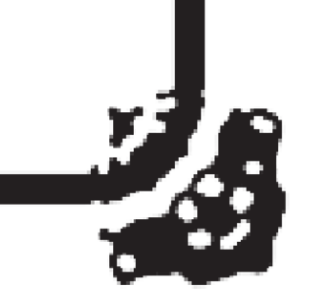
\includegraphics[width=0.4\textwidth]{image/introduction/inverse-design-bend.png}
  }

  % 2° row
  % Traditional splitter
  \subfigure[\emph{Splitter} con diseño tradicional.]{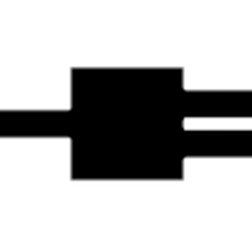
\includegraphics[width=0.4\textwidth]{image/introduction/traditional-splitter.png}}
  \hfill
  % Inverse design splitter
  \subfigure[WDM obtenido con diseño inverso. Extraído de \citep{Su2020}.]{
    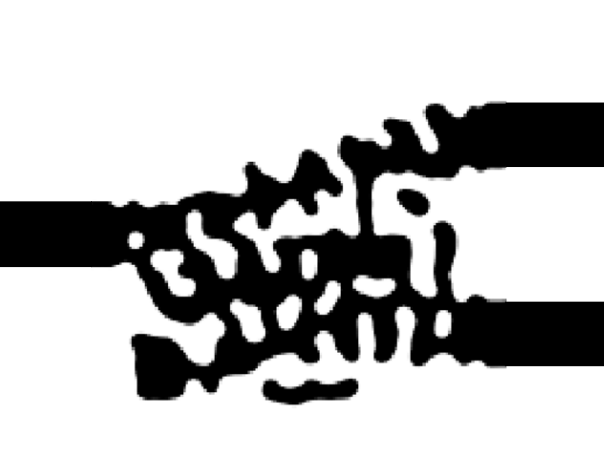
\includegraphics[width=0.4\textwidth]{image/introduction/inverse-design-splitter.png}
  }

  \caption{Diseños tradicionales y obtenidos a partir de diseño inverso de un
  \emph{bend} y un WDM.}
  \label{fig:devices}

\end{figure}


La \autoref{fig:devices} presenta una comparación de dos metodologías de diseño: tradicional e inverso.
Como se observa en la \autoref{fig:devices}, en el diseño tradicional (izquierda) se define el dispositivo con geometrías simples que permiten obtener funciones analíticas de sus propiedades físicas \citep{Hughes2016, Song2008}. 
Esto se realiza para poder optimizar la función obtenida a partir de los parámetros que la definan. 
Dicha optimización se suele ejecutar haciendo un barrido de los parámetros, con algoritmos genéticos o usando \emph{particle swarm optimization}. 
Para obtener buenos resultados con esta metodología comúnmente se requiere intuición 
y/o conocimiento de un experto sobre el tema \citep{Su2020}. 


Existen tres grandes inconvenientes con el diseño tradicional. 
Primero, solamente se explora una pequeña fracción de todos los posibles diseños.
Segundo, por lo general no es conocido el límite de rendimiento del dispositivo
\citep{Molesky2018}.
Tercero, al trabajar en la escala de nanómetros, existen casos como el
\emph{bend-90°} y \emph{wavelength-demultiplexer} que presentan un bajo rendimiento con diseños tradicionales \citep{Su2020}.

Por otro lado, en el diseño inverso, mostrado en la \autoref{fig:devices}
(derecha), las geometrías resultantes no están limitadas a diseños intuitivos o regulares.
Esta metodología consiste en primero definir que propiedades deseamos en nuestro dispositivo.
Luego, usando simulaciones computacionales podemos determinar las propiedades físicas
de una geometría arbitraria. De este modo, el problema se reduce a parametrizar una región
de diseño y explorar distintas geometrías con esta parametrización hasta encontrar un diseño
que cumpla las propiedades deseadas.
Esto se formula como un problema de optimización, para lo cual existe una variedad de algoritmos
que se pueden aplicar (e.g. \emph{genetic algorithms}, \emph{particle swarm optimization}, etc)
\citep{Molesky2018, Su2020}.
Para una descripción detallada de los distintos algoritmos de optimización
comúnmente empleados, por favor revisar \cite{Schneider2019, Elsawy2020, Campbell2019}.


El diseño inverso ha logrado conseguir dispositivos con menores pérdidas que las obtenidas por el
diseño tradicional por lo que ha ganado interés en el área de fotónica durante
las últimas dos décadas \citep{Su2018, Molesky2018, Campbell2019}. 
Sin embargo, existen cuatro grandes desafíos con este planteamiento:
(i) el espacio de búsqueda es exponencial \citep{Vuckovic2019}, 
(ii) las simulaciones computacionales son costosas en términos de tiempo y memoria \citep{Kudyshev2020}, 
(iii) el espacio de búsqueda es no convexo \citep{Su2018} y
(iv) no todos los diseños son fabricables \citep{Su2020}.


El presente trabajo se centra en estudiar dos dispositivos SiP
fundamentales:
(i) \emph{bend-90°} y (ii) \emph{wavelength demultiplexer} de dos canales.
De aquí en adelante nos referiremos a estos simplemente como \emph{bend} y WDM.
Así, el objetivo de esta tesis es aplicar el conocimiento en computación para
encontrar diseños de estos dispositivos con eficiencias mayores al 90\%
y resilientes a errores de fabricación trabajando en la escala de nanómetros.
Empleamos el diseño inverso para encontrar los diseños que cumplían estas propiedades,
realizamos una parametrización topológica para explorar los posibles diseños.
El estudio se realizó con cinco algoritmos de optimización populares en el área.
Además, se incorporaron restricciones a los diseños para asegurar robustez al fabricarse.

El presente documento está organizado de la siguiente manera:

El \autoref{chapter:introduction}  brinda una introducción al tema de investigación, describe el problema a detalle, justifica la relevancia de resolverlo, define los objetivos y señala los aportes del trabajo.

El \autoref{chapter:theory} desarrolla los conceptos necesarios para entender la propuesta presentada
en esta tesis.

El \autoref{chapter:related-works} presenta una revisión del estado del arte centrándose
en algoritmos utilizados en el diseño inverso y dos estrategias populares de parametrización:
(i) basada en conjuntos de nivel y (ii) basada en píxeles.

El \autoref{chapter:methodology} plantea los pasos seguidas en este trabajo y brinda
todos los detalles necesarios para que puedan ser reproducibles.

El \autoref{chapter:results} muestra los resultados de la experimentación seguida.
Además, contiene una discusión crítica de los resultados junto a un análisis de los
diseños mejor optimizados.

Por último, en el \autoref{chapter:conclutions} se detallan las conclusiones del presente trabajo de investigación.

\section{Descripción del Problema}

Una forma de parametrizar dispositivos es seleccionando una región rectangular y dividiéndola
en $n \times m$ píxeles como si fuera una imagen, ver \autoref{fig:bend-discretization}.
Luego, cada píxel se rellena con dos posibles materiales: óxido de silicio $(SiO_2)$ o Silicio ($Si$).
Finalmente, se usa métodos numéricos para resolver las ecuaciones de Maxwell en este diseño
y obtener así la distribución del campo eléctrico, este permite entender el funcionamiento del dispositivo
y sus propiedades \citep{Molesky2018, Schneider2019}.

\begin{figure}[ht]
  \centering
  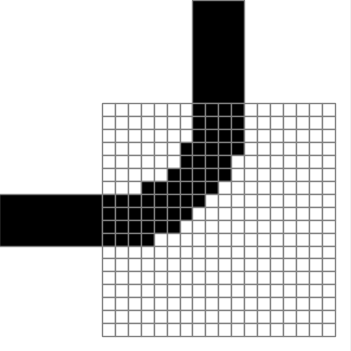
\includegraphics[scale=0.6]{image/introduction/bend-discretization.png}
  \caption{\emph{Bend} con una región de diseño discretizada en $18 \times 18$
  píxeles. Cada píxel negro representa la presencia de $Si$ y cada píxel blanco
  de $SiO_2$.}
  \label{fig:bend-discretization}
\end{figure}

Con esta parametrización, el diseño inverso comienza definiendo los requerimientos del dispositivo para luego tratar de buscar entre los $2^{n \times m}$ posibles diseños algún candidato que se adapte a lo que se busca \citep{Su2020, Molesky2018}.
Como prueba de concepto, trabajos como el de \cite{Malheiros-Silveira2020} parametrizaron $2^{10 \times 10}$ posibles geometrías.
Pero, se presentan algunas dificultades con esta estrategia:

\begin{enumerate}
  \item No es viable evaluar todos los posibles diseños por haber un número excesivamente elevado de ellos \citep{Vuckovic2019}.
  \item Las simulaciones computacionales son muy costosas en términos de consumo de memoria y 
    tiempo de ejecución \citep{Kudyshev2020}.
  \item El espacio de búsqueda es no convexo \citep{Su2018}.
  \item No todos los diseños son fabricables por limitaciones físicas \citep{Su2020}.
  \item Cada dispositivo es una clase distinta de problema, es decir, no necesariamente funcionará la misma estrategia para cada dispositivo \citep{Molesky2018}.
\end{enumerate}

Además, la fabricación viene con otros desafíos, principalmente:

\begin{enumerate}
  \item Errores de precisión en los instrumentos \citep{Piggott2017}.
  \item Sensibilidad ante cambios de temperatura \citep{Vuckovic2019}.
\end{enumerate}

Considerando las anteriores dificultades, el problema es usar diseño inverso y encontrar geometrías que muestren buen desempeño en simulaciones computacionales y que puedan asegurar mantener un óptimo funcionamiento al ser fabricados. 
Este problema se estudió para dos dispositivos nanofotónicos (i) \emph{bend} y (ii) WDM.

\section{Justificación}

El \emph{bend} y WDM son dispositivos SiP fundamentales que tienen aplicación
directa, por ejemplo, en sistemas HPC \citep{Shen2017}.
Así, las mejoras de estos ayudará indirectamente al desarrollo de Ciencia
de la Computación brindando, potencialmente, un mejor \emph{hardware} para programas de
inteligencia artificial, HPC, entre otros.
Por otro lado, desde el punto de vista computacional, 
este problema es interesante porque ya hay estrategias computacionales conocidas para resolverlo;
por ejemplo, algoritmos genéticos \citep{Mykel2019}, estrategias evolutivas \citep{Hansen2016}, entre otros.
Además, debido al alto costo computacional de las simulaciones \citep{Schneider2019}, el trabajo requiere de computación de alto desempeño.

\section{Objetivos}

\begin{itemize}

  \item Diseñar un \emph{bend} y WDM con eficiencias mayores al 90\% y resiliente a errores de fabricación.

  \begin{itemize}

    \item Seleccionar una estrategia de parametrización que asegure facilidad de fabricación.

    \item Definir una función objetivo que encapsule las propiedades buscadas en cada dispositivo.

    \item Encontrar geometrías con valores óptimos de la función objetivo en simulaciones computacionales.

    \item Encontrar geometrías resilientes a posibles errores de fabricación de dilatación o contracción.

  \end{itemize}

  \item Comparar el desempeño y la convergencia de cinco algoritmos de optimización populares usados para optimizar dispositivos nanofotónicos.

\end{itemize}
